% TeXLocal test document: Beamer slides.
%
% What to try with it:
%  - Wide pages: Fit Width, Fit Height and zoom on 16:9 slides.
%  - Overlays (\pause, \only, \item<n->) make one frame several pages;
%    SyncTeX from any of them goes back to the frame.
%  - The outline lists the slides' sections and subsections.
\documentclass[aspectratio=169]{beamer}
\usetheme{Madrid}
\usepackage{tikz}

\title{Test Slides}
\subtitle{For TeXLocal}
\author{The TeXLocal Test Documents}
\date{\today}

\begin{document}

\begin{frame}
  \titlepage
\end{frame}

\begin{frame}{Contents}
  \tableofcontents
\end{frame}

\section{Overlays}

\begin{frame}{Pausing}
  First point.
  \pause
  Second point, on the next page.
  \pause
  Third point, on the page after.
\end{frame}

\begin{frame}{Items One at a Time}
  \begin{itemize}
    \item<1-> Always shown
    \item<2-> From the second step
    \item<3-> From the third step
    \item<4-> From the fourth step
  \end{itemize}
\end{frame}

\subsection{Alternatives}
\begin{frame}{Only and Uncover}
  \only<1>{Shown only on the first step.}
  \only<2>{Shown only on the second step.}
  \uncover<3>{Uncovered on the third step, reserved space before.}
\end{frame}

\section{Content}

\begin{frame}{Blocks}
  \begin{block}{A Block}
    Some text in a block.
  \end{block}
  \begin{alertblock}{An Alert}
    Something to notice.
  \end{alertblock}
  \begin{exampleblock}{An Example}
    $e^{i\pi} + 1 = 0$
  \end{exampleblock}
\end{frame}

\begin{frame}{Columns}
  \begin{columns}
    \begin{column}{0.5\textwidth}
      \begin{itemize}
        \item Left column
        \item With a list
      \end{itemize}
    \end{column}
    \begin{column}{0.5\textwidth}
      \centering
      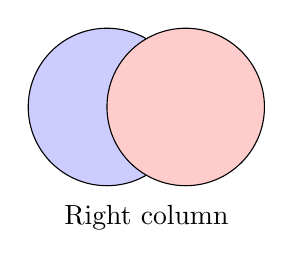
\begin{tikzpicture}
        \draw[fill=blue!20] (0,0) circle (1);
        \draw[fill=red!20] (1,0) circle (1);
        \node at (0.5,-1.4) {Right column};
      \end{tikzpicture}
    \end{column}
  \end{columns}
\end{frame}

\subsection{Mathematics}
\begin{frame}{An Equation}
  \[
    \sum_{k=1}^{n} k = \frac{n(n+1)}{2}
  \]
  \pause
  \[
    \sum_{k=1}^{n} k^2 = \frac{n(n+1)(2n+1)}{6}
  \]
\end{frame}

\section{Wrapping Up}

\begin{frame}{Summary}
  \begin{enumerate}
    \item Overlays make pages.
    \item Blocks and columns lay out a slide.
    \item This is the last slide.
  \end{enumerate}
\end{frame}

\end{document}
